%%%%%%%%%%%%%%%%%%%%%%%%%%%%%%%%%%%%%%%%%%%%%%%%%%%%%%%%%%%%%%%%%%%%%%%%%%%%%
%
% Bayesian prediction of luminosity distribution based on one simulation run:
% An example from TARDIS
%
%%%%%%%%%%%%%%%%%%%%%%%%%%%%%%%%%%%%%%%%%%%%%%%%%%%%%%%%%%%%%%%%%%%%%%%%%%%%%
\documentclass[11pt]{article}
\usepackage[utf8]{inputenc}

\usepackage[a4paper, left=20mm, right=20mm, top=25mm, bottom=25mm]{geometry}
\usepackage[numbers]{natbib}
\usepackage{hyperref}
\usepackage{physics}

\usepackage[colorinlistoftodos]{todonotes} % Use 'disable' to remove todos in final version
\newcommand{\fred}[1]{\todo[color=orange!40,inline]{#1}} %
\newcommand{\fredmargin}[1]{\todo[color=orange!40]{#1}} %
\newcommand{\checked}{\todo[color=green,noline]{\checkmark}} %
\newcommand{\checkedl}{\todo[color=brown]{\checkmark}} %
\newcommand{\hans}[1]{\todo[color=yellow!30,inline]{#1}} %
\newcommand{\hanslong}[2][]{\todo[%bordercolor=red,
  color=white,inline,caption={2do}, #1]{
    \begin{minipage}{\textwidth} #2\end{minipage}}} %

%% CHANGE THIS DATE AS YOU MODIFY THE FILE
\newcommand{\vdate}{161206}
\pagestyle{myheadings}
\markboth{Version \vdate} {Version \vdate}

\parindent=3ex
%%%%%%%%%%%%%%%%%%%%%%%%%%%%%%%%%%%%%%%%%%%%%%%%%%%%%%%%%%%%%%%%%%%%%%%%%%%%%
\usepackage{bm,amssymb,amsfonts,amsmath}  % bold math symbols, AMStex
\usepackage{graphicx}    % standard graphics
%%%%%%%%%%%%%%%%%%%%%%%%%%%%%%%%%%%%%%%%%%%%%%%%%%%%%%%%%%%%%%%%%%%%%%%%%%%%%
\newcommand{\lleq}[1]{\label{#1} }
% TO REMOVE THE LABEL LETTERS FROM THE EQUATION DISPLAY, COMMENT OUT THIS LINE:
\renewcommand{\lleq}[1]{\label{#1} {\scriptstyle {\rm (#1)}} \hspace*{2ex} }

\newcommand{\smA}{{\scriptscriptstyle A}}
\newcommand{\smB}{{\scriptscriptstyle B}}
\newcommand{\smH}{{\scriptscriptstyle H}}
\newcommand{\smK}{{\scriptscriptstyle K}}
\newcommand{\smL}{{\scriptscriptstyle L}}
\newcommand{\smM}{{\scriptscriptstyle M}}
\newcommand{\smN}{{\scriptscriptstyle N}}
\newcommand{\smR}{{\scriptscriptstyle R}}

\newcommand{\smo}{{\scriptscriptstyle 1}}
\newcommand{\smt}{{\scriptscriptstyle 2}}
\newcommand{\smr}{{\scriptscriptstyle 3}}
\newcommand{\smf}{{\scriptscriptstyle 4}}
\newcommand{\smv}{{\scriptscriptstyle 5}}
\newcommand{\smx}{{\scriptscriptstyle 6}}
\newcommand{\sms}{{\scriptscriptstyle 7}}
\newcommand{\sme}{{\scriptscriptstyle 8}}
\newcommand{\smn}{{\scriptscriptstyle 9}}

\newcommand{\bma}{{\bm{a}}}
\newcommand{\bmb}{{\bm{b}}}
\newcommand{\bmc}{{\bm{c}}}
\newcommand{\bmd}{{\bm{d}}}
\newcommand{\bme}{{\bm{e}}}
\newcommand{\bmf}{{\bm{f}}}
\newcommand{\bmg}{{\bm{g}}}
\newcommand{\bmh}{{\bm{h}}}
\newcommand{\bmi}{{\bm{i}}}
\newcommand{\bmj}{{\bm{j}}}
\newcommand{\bmk}{{\bm{k}}}
\newcommand{\bml}{{\bm{\ell}}}
\newcommand{\bmm}{{\bm{m}}}
\newcommand{\bmn}{{\bm{n}}}
\newcommand{\bmo}{{\bm{o}}}
\newcommand{\bmp}{{\bm{p}}}
\newcommand{\bmq}{{\bm{q}}}
\newcommand{\bmr}{{\bm{r}}}
\newcommand{\bms}{{\bm{s}}}
\newcommand{\bmt}{{\bm{t}}}
\newcommand{\bmu}{{\bm{u}}}
\newcommand{\bmv}{{\bm{v}}}
\newcommand{\bmw}{{\bm{w}}}
\newcommand{\bmx}{{{\bm{x}}}}
\newcommand{\bmy}{{\bm{y}}}
\newcommand{\bmz}{{\bm{z}}}
\newcommand{\bmA}{{\bm{A}}}
\newcommand{\bmB}{{\bm{B}}}
\newcommand{\bmC}{{\bm{C}}}
\newcommand{\bmD}{{\bm{D}}}
\newcommand{\bmE}{{\bm{E}}}
\newcommand{\bmF}{{\bm{F}}}
\newcommand{\bmG}{{\bm{G}}}
\newcommand{\bmH}{{\bm{H}}}
\newcommand{\bmI}{{\bm{I}}}
\newcommand{\bmJ}{{\bm{J}}}
\newcommand{\bmK}{{\bm{K}}}
\newcommand{\bmL}{{\bm{L}}}
\newcommand{\bmM}{{\bm{M}}}
\newcommand{\bmN}{{\bm{N}}}
\newcommand{\bmO}{{\bm{O}}}
\newcommand{\bmP}{{\bm{P}}}
\newcommand{\bmQ}{{\bm{Q}}}
\newcommand{\bmR}{{\bm{R}}}
\newcommand{\bmS}{{\bm{S}}}
\newcommand{\bmT}{{\bm{T}}}
\newcommand{\bmU}{{\bm{U}}}
\newcommand{\bmV}{{\bm{V}}}
\newcommand{\bmW}{{\bm{W}}}
\newcommand{\bmX}{{\bm{X}}}
\newcommand{\bmY}{{\bm{Y}}}
\newcommand{\bmZ}{{\bm{Z}}}

\newcommand{\bmalpha}{{\bm{\alpha}}}
\newcommand{\bmbeta}{{\bm{\beta}}}
\newcommand{\bmchi}{{\bm{\chi}}}
\newcommand{\bmdelta}{{\bm{\delta}}}
\newcommand{\bmepsilon}{{\bm{\varepsilon}}}
\newcommand{\bmphi}{{\bm{\phi}}}
\newcommand{\bmgamma}{{\bm{\gamma}}}
\newcommand{\bmeta}{{\bm{\eta}}}
\newcommand{\bmiota}{{\bm{\iota}}}
\newcommand{\bmkappa}{{\bm{\kappa}}}
\newcommand{\bmlambda}{{\bm{\lambda}}}
\newcommand{\bmmu}{{\bm{\mu}}}
\newcommand{\bmnu}{{\bm{\nu}}}
\newcommand{\bmomega}{{\bm{\omega}}}
\newcommand{\bmpi}{{\bm{\pi}}}
\newcommand{\bmpsi}{{\bm{\psi}}}
\newcommand{\bmrho}{{\bm{\rho}}}
\newcommand{\bmsigma}{{\bm{\sigma}}}
\newcommand{\bmtau}{{\bm{\tau}}}
\newcommand{\bmtheta}{{\bm{\theta}}}
\newcommand{\bmupsilon}{{\bm{\upsilon}}}
\newcommand{\bmxi}{{\bm{\xi}}}
\newcommand{\bmzeta}{{\bm{\zeta}}}


\newcommand{\hypo}  {{\mathcal{H}}}  % Model
\newcommand{\ldef}{\;{:}{=}\;}
\newcommand{\rdef}{\;{=}{:}\;}
\newcommand{\realnumbers}{\mathbb{R}}
\newcommand{\integers}{\mathbb{Z}}
\newcommand{\cond}{\,|\,}
\newcommand{\NBD}{\mathrm{NB}}

\newcommand{\refeq}[1]{Eq.~(\ref{#1})}
\newcommand{\reffig}[1]{Fig.~\ref{fig:#1}}
\newcommand{\refsec}[1]{Sec.~\ref{sec:#1}}

\DeclareMathOperator{\Expect}{\mathbb{E}}
\newcommand{\expect}[1]{\Expect\left[#1\right]}
\newcommand{\expectest}[1]{\widehat{\Expect\left[#1\right]}}
\DeclareMathOperator{\GammaDist}{Gamma}
\DeclareMathOperator{\GaussianDist}{\mathcal{N}}
\DeclareMathOperator{\InvGammaDist}{InvGamma}
\newcommand{\Kalpha}{{K_\alpha}}
\newcommand{\Kbeta}{{K_\beta}}
\newcommand{\npack}{{n_p}}
\newcommand{\lmax}{\ell_{\rm max}}
\newcommand{\Lmax}{{L_{\rm max}}}
\newcommand{\Lumtot}{Q}
\newcommand{\lumtot}{q}
\newcommand{\Lum}{L}
\newcommand{\lum}{\ell}
% \newcommand{\rmdx}[1]{\mbox{d} #1 \,} % differential
\newcommand{\rmdx}[1]{\dd{#1}} % differential
\newcommand{\firstDeriv}[1]{\frac{\partial}{\partial #1}}
\newcommand{\secDeriv}[1]{\frac{\partial^2}{\partial #1^2}} % second partial derivative
\newcommand{\secPartial}[2]{\frac{\partial^2}{\partial #1 \, \partial #2}} % second partial derivative
\newcommand{\tardis}{TARDIS}
\DeclareMathOperator{\Variance}{\mathbb{V}}
\newcommand{\variance}[1]{\Variance\left[#1\right]}

%%%%%%%%%%%%%%%%%%%%%%%%%%%%%%%%%%%%%%%%%%%%%%%%%%%%%%%%%%%%%%%%%%%%%%%%%%%%%
\begin{document}

\begin{center}
  \textbf{\Large Bayesian prediction of supernova luminosity  distributions}\\[8pt]
  \textbf{\Large based on simulation output}\\[12pt]
\end{center}

\textbf{Abstract} TODO\\

\section{What's left to do}

\subsection{why asymptotic approx. has larger variance}
\begin{enumerate}
  \item For $\alpha=1.5, \beta=60, n=14000$ still get 50 \% larger uncertainty from asymptotic compared to summation over $N$. Is it due very asymmetric one-packet distribution? Try larger $\alpha$, for example $\alpha = 30$.
  \item  Another option: $\int \rmdx{\alpha} \rmdx{\beta}$, use true values in simulation. Where does uncertainty come from? From $\lambda$ or $\mu, \sigma^2$?
  \item Are finite number of terms in $\sum_N$ a problem? Check

\end{enumerate}

\subsection{Plots}

\begin{enumerate}
  \item generate a toy spectrum, take frequencies from actual tardis,
  generate luminosities from a $\GammaDist(\alpha, \beta)$, no $\nu$
  dependence of $\alpha, \beta$ for clarity , plot spectrum with
  uncertainty bands, show it early in the paper, then describe where
  it comes from
  \item compare asymptotic and $\sum_N$ $p(\Lumtot \cond \bmy)$ on a
  plot, add what happens if only $\sqrt{n}$ uncertainty is used: that
  would neglect uncertainty on the single-packet distribution, show
  case when parameters determined from a single bin with few samples,
  should make large difference. Fix $\lambda$, what are the uncertainties now?
  \item Statistics of replicas: again compare \refeq{spe} to \refeq{ral}. Teach a lesson: from a single data set, prediction will be centered there
  \item Question: does Wolfgang want to see a plot in which ``$\lambda$ is divided out''? That is , just plot how mean
\end{enumerate}

\subsection{Other issues that need to be resolved}

\begin{enumerate}

\item Clean up integrals using \verb=\rmdx= rather than $d$.

\item Write everything in terms of frequency $\nu$ or wavelength
  $\lambda$

\item Now that we have removed direct analysis of \tardis\ from the
  paper, there is no need to define an overall parameterization of the
  Gamma parameters $\alpha(\nu_b) = \sum_k a_k \nu_b^k$ and
  $\beta(\nu_b) = \sum_k b_k \nu_b^k$. However, the possibility of
  linking the analyses of all the bins by this and similar methods
  should be highlighted. Perhaps in the Conclusions?

\item \textbf{\tardis} move tardis section into separate document in
  this git repo. Better to keep it out of the paper. Cite tardis when
  showing the toy spectrum. Mention that in reality $\alpha$ and
  $\beta$ are $\nu$ dependent

\end{enumerate}


\section{Introduction (Wolfgang)}

\subsection{Astrophysical context}

Wolfgang's text

\subsection*{Main points of this paper}

\begin{enumerate}
\item The first goal of this paper is to show that the Bayesian
  approach to this problem is well-founded and robust.

\item Luminosity data generated by a single simulation provide a
  basis for predicting its uncertainty, i.e.\ how much this luminosity
  can be expected to vary from simulation to simulation.

\item The uncertainty in the luminosity calculated in the Bayesian
  approach is larger than anticipated because it takes into account
  not only the variability of the luminosity per packet, but also the
  distribution of the number of packets.

\item Traditional methods using conventional counting ratios
  (``relative frequencies'') can also make predictions for such
  uncertainties, but only if the number of packets is large. By
  contrast, the Bayesian method presented here remains valid also for
  small packet multiplicities.

\end{enumerate}

%%%%%%%%%%%%%%%%%%%%%%%%%%%%%%%%%%%%%%%%%%%%%%%%%%%%%%%%%%%%%%%%%%%%%%%%%%%%%
\subsection{Bayesian prediction}
\label{sec:bayp}

We first sketch the generic notation and relations for Bayesian
probability theory.
%
A particular experiment or simulation generates
\textit{data}
which will often come in the form of a list of $n$ measurements,
$\bmy = (y_1,y_2,\ldots,y_n)$. In order to understand or explain these
data, the observer constructs one or more \textit{models} or
\textit{hypotheses} $\hypo$. Central to this construction is the
specification of a \textit{likelihood} $p(\bmy\cond \bmtheta,\hypo)$
where $\bmtheta = (\theta_1,\theta_2,\ldots,\theta_K)$ is the set of
unknown parameters specified by the model. The likelihood is the
probability assigned by the model $\hypo$ to the data $\bmy$ when the
parameters $\bmtheta$ are fixed and known.
%
If and when the individual measurements $y_i$ are independent, the
joint likelihood is the product
\begin{align}
  \lleq{bta}
  p(\bmy\cond \bmtheta) &= \prod_{i=1}^n p(y_i\cond \bmtheta).
\end{align}
At this level of analysis, the goal is to find which values for these
parameters provide a satisfactory description of the data. In the
Bayesian context, these parameter values are best described in terms
of the probability of the parameters given the data,
$p(\bmtheta\cond \bmy)$. This so-called \textit{posterior} is related
to the likelihood by Bayes' Theorem,
\begin{align}
  \lleq{bth}
  p(\bmtheta\cond \bmy)
  &= \frac{p(\bmy\cond\bmtheta)\;p(\bmtheta)}
    {p(\bmy)}
    %= \frac{p(\bmy\cond\bmtheta)\;p(\bmtheta)}
    %{\int \rmdx{\bmtheta}'\, p(\bmy\cond\bmtheta')\;p(\bmtheta')}
\end{align}
where $p(\bmtheta)$, the so-called \textit{prior}, is the probability
assigned to the values of the parameters before any data were taken
into account and the \textit{evidence}
\begin{align}
  \lleq{bti}
  p(\bmy) &= \int \rmdx{\bmtheta}'\, p(\bmy\cond\bmtheta')\;p(\bmtheta'),
\end{align}
is fully determined by the likelihood and prior.
%
Prediction of any ``future'' data $Y$ is made not by considering the
likelihood $p(Y\cond\bmtheta_{\rm max})$ using single
maximum-likelihood parameter values $\bmtheta_{\rm max}$, but by
integrating over all possible values of the likelihood, weighted by
the posterior,
\begin{align}
  \lleq{btj}
  p(Y\cond \bmy) &= \int \rmdx{\bmtheta}\,p(Y\cond\bmtheta)\,p(\bmtheta\cond \bmy).
\end{align}
The above relations are true for any type of data and can be applied
to actual experimental data and the pertinent physical parameters. The
scope of this paper, however, is limited to the relationship between
simulated data generated by radiative transfer simulation codes.
Likewise, all parameters considered below relate strictly to model
descriptions of the simulation.

%%%%%%%%%%%%%%%%%%%%%%%%%%%%%%%%%%%%%%%%%%%%%%%%%%%%%%%%%%%%%%%%%%%%%%%%%%%%%
\section{Single-simulation data and multi-simulation prediction}

% \subsection{Output data from radiative transfer simulations}
% \subsection{Simulation data}

We consider a single computer simulation which generates a luminosity
spectrum from $\npack$ photon packets, each having a particular
frequency $\nu_i$ and luminosity $\lum_i$. Together, these frequencies
and luminosities form the raw simulation data
$\bmy = \{ (\nu_i,\lum_i): i = 1,\ldots,\npack\}$.  We divide up the
frequency spectrum into bins of width $\Delta\nu$ centered on
frequencies $\nu_b$ resulting in bin intervals
$\Delta_b = [\nu_b {-} \tfrac{1}{2} \Delta\nu \,,\, \nu_b {+}
\tfrac{1}{2} \Delta\nu], b = 1,2,\ldots, B$. Let $n_b$ be the number
of packets having a frequency falling into a particular bin $b$, and
let the vector $\bml_b = \{(\ell_{b,j}): j = 1,\ldots,n_b\}$ be the
set of luminosities of those packets. The data set is correspondingly
cast into the more compact histogram form
\begin{align}
  \lleq{sdb}
  \bmy = \{(n_b,\bml_b): b = 1,\ldots,B\}
\end{align}
with loss of information limited to replacing the exact packet
frequencies $\nu_i$ by the approximate bin frequency $\nu_b$. The
total luminosity in bin $b$ is
\begin{align}
  \lleq{sdc}
  \lumtot_b
  &= \sum_{j=1}^{n_b} \lum_{b,j}.
\end{align}
Within a given model $\hypo$, the data $\bmy$ are only one of many
possible realisations of the corresponding random variables; for
example, starting the simulation with a different seed would result in
different output data. We denote the general random variables by the
corresponding upper-case symbols,
\begin{align}
  \lleq{sdd}
  \bmL_b &= \{(\Lum_{b,j}): j = 1,\ldots,N_b\}\\
  \lleq{sde}
  \bmY &= \{(N_b, \bmL_b): b = 1,\ldots,B\},\\
  \lleq{sdf}
  \Lumtot_b &= \sum_{j=1}^{N_b} \Lum_{b,j},
\end{align}
Lower-case symbols such as $\bmy, n_b,\bml_b$ etc.\ are strictly
reserved for the simulated data at hand.


The goal of this paper is to illustrate how the single-simulation data
$\bmy$ can be used to predict the distribution of total bin
luminosities $Q_b, b = 1,\ldots,B$ if many simulations had been
carried out. At this introductory level, we assume that the different
luminosities are independent, so that the prediction of the entire
spectrum (including all its uncertainty) is the product of predictions
for each frequency bin,
\begin{align}
  \lleq{sdg}
  p(Q_1,Q_2,\ldots,Q_B\cond\bmy) = \prod_{b=1}^B p(Q_b\cond \bmy).
\end{align}

\section{The generic model} \label{sec:model}

Various physical processes such as absorption result in luminosity
spectra with strong features. The model we develop below takes into
account the variability introduced by these features in a two-step
process termed a \textit{compound process} in the statistics
literature.
%
In the first step, the number of packets $N$ is modelled by means of a
separate Poisson distribution $p(N\cond\lambda)$ for each bin, where
the magnitude of $\lambda$ will capture most of the variability of the
spectrum. Given $N$, the single-packet luminosity distribution is
modelled in the second step by means of a packet likelihood for
$\Lum_{b,j}$ with packet parameters, a packet prior and, of course,
packet parameter posterior. The single-packet distribution contains
the crucial information which allows us to extend previous methods to
cases where the number of packets in a bin is small.
%%%%%%%%%%%%%%%%%%%
\fred{Refs: Zech, maybe others, too}


We derive in this section the generic equations of the compound
process, and then proceed to show in Sections \ref{sec:example} and
\ref{sec:asymptotic} how these equations can be used in two different
ways.
%
We consider for the moment quantities in one bin $b$ only, and hence
drop the $b$-subscripts, e.g.\
$Q_b \to Q, n_b \to n, N_b\to N, \bml_b\to\bml, L_{b,j} \to L_j$ etc.


We seek a Bayesian prediction for the total luminosity in one bin,
$p(Q\cond n,\bml)$, one of the factors in Eq.~(\ref{sdg}).  To do so,
we must take into account all possible values of variables and
parameters entering our model.  This involves multiple use of the
\textit{marginalisation rule}, which states that, to obtain the
probability for a variable $U$ when we are not interested in another
variable $V$, the marginal probability for $U$ is %
$p(U) = \int dV\,p(U,V) = \int dV\,p(U\cond V)\,p(V)$ for continuous
$V$ and $p(U) = \sum_V p(U,V) = \sum_V p(U\cond V)\,p(V)$ for discrete
$V$ respectively.
%
The uninteresting variables $V$ in the present case are the number of
packets $N$, the set of luminosities $\bmL$ of the $N$ packets
whose likelihood is modelled by a distribution determined by
likelihood parameters $\bmphi$,
\begin{align}
  \lleq{slk}
  p(\bmL\cond N,\bmphi)
  &= \prod_{j=1}^{N} p(L_j\cond \bmphi)
\end{align}
and the parameter $\lambda$ governing the likelihood for the number of
packets, $p(N\cond\lambda)$. Multiple use of the marginalisation rule
on $p(Q\cond n,\bml)$ results in
\begin{align}
  \lleq{sll}
  p(Q\cond n,\bml)
  &= \sum_{N=0}^\infty \;\int_0^\infty \rmdx{\lambda}\;
    p(N\cond\lambda)\;
    p(\lambda\cond n)
    \int \rmdx{\bmL}\;
    p(Q\cond N,\bmL)\;
    \int \rmdx{\bmphi}\;
    p(\bmL\cond N,\bmphi)\,
    p(\bmphi\cond n,\bml),
\end{align}
where we have omitted from the probabilities all quantities to the
right of the conditional line which are irrelevant to the variable at
hand. For example, Eq.~(\ref{sdf}) shows that the total bin luminosity
$Q$ is fully determined by $N$ and $\bmL$ and so we can shorten
$p(Q\cond N,\bmL,\lambda,\bmphi,n,\bml)$ to $p(Q\cond N,\bmL)$. %
Likewise the probability for $\bmL$ is fully determined by $N$ and the
parameters $\bmphi$ and does not depend on the data $n,\bml$.  The
bounds of $\int \rmdx{\bmL}$ and $\int \rmdx{\bmphi}$ are determined by the
specific model and data for which $p(Q\cond n,\bml)$ is to be
calculated.
%
We note that a part of Eq.~(\ref{sll}) can be seen as a convolution
since $p(Q\cond N,\bmL)$ can be written as a Dirac delta function,
\begin{align}
  \lleq{slm}
  \int \rmdx{\bmL}\; p(Q\cond N,\bmL)\; p(\bmL\cond N,\bmphi)
  &= \int \rmdx{\bmL}\;\delta(Q - \textstyle\sum_{j=1}^N L_j)\; \prod_j p(L_j\cond \bmphi).
\end{align}
Eq.~(\ref{sll}) is exact, and in principle all that remains is to make
specific choices for the various probabilities which are judged best
to represent the data at hand, and thence to carry out the sum and
multiple integrals. In practice, of course, such calculations may be
time-consuming, and there will often be more than one choice for the
functional form of each probability. In Section \ref{sec:example}, we
shall therefore set out a specific example


\section{Example A: modelling single-packet luminosity distributions}
\label{sec:example}

In this section, we show by example how information on the
single-packet luminosity distributions can be utilised to find exact
expressions for Eq.~(\ref{sll}).

\subsection{Multiplicity prediction}

First, the parameter $\lambda$ is eliminated as follows. The number of
packets $N$ is Poisson-distributed
\begin{align}
  \lleq{pmb}
  p(N\cond\lambda) &= \frac{e^{-\lambda}\lambda^{N}}{N!}
  \quad N = 0,1,\ldots,\infty.
\end{align}
The observed $n$ is naturally presumed to have arisen from the same Poisson
distribution with the same $\lambda$, so $p(n\cond\lambda) =
e^{-\lambda}\lambda^{n}/n!$. %
% and since $n$ is just one realisation of $N$, it likewise is
% poissonian $p(n\cond\lambda) = e^{-\lambda}\lambda^{n}/n!$ with the
% same $\lambda$.
The posterior for $\lambda$ is found from the data $n$ via Bayes'
Theorem,
\begin{align}
  \lleq{pmc}
  p(\lambda\cond n) %
  &= \frac{p(n\cond\lambda)\,p(\lambda)} {p(n)}
  \ =\ \frac{p(n\cond\lambda)\,p(\lambda)} %
  {\int \rmdx{\lambda} p(n\cond\lambda)\,p(\lambda)} \,.
\end{align}
We use an improper prior
\begin{align}
  \lleq{pmf}
  p(\lambda) = c \lambda^{-a},
\end{align}
meaning that $\int_0^\infty \rmdx{\lambda}\,p(\lambda)$ is known only up to
a constant $c$. A hyperparameter choice $a=0$ yields the uniform
prior, $a=1/2$ gives the Jeffreys and reference prior, and $a=1$ is
the transformation-group result advocated by
Jaynes~\cite[Ch. 12]{jaynes2003probability}. An improper prior is not
a problem because $c$ cancels out when calculating the posterior,
provided that $n \ge 1$; i.e., at least one packet is observed in the
bin.\footnote{For a uniform prior, the case $a{=}0$, we require of
  course a parameter $\lambda_{\rm max}$. As long as
  $\lambda_{\rm max}$ is large enough, it too would cancel.}, The
posterior is
\begin{align}
  \lleq{pms}
  p(\lambda\cond n)
  &= \GammaDist(\lambda \cond \alpha = n{-}a{+}1 \,,\, \beta = 1)\,,
\end{align}
where the $\GammaDist$ distribution with shape parameter $\alpha > 0$ and
rate parameter $\beta > 0$ is defined as
\begin{align}
  \lleq{gma}
  \GammaDist(x\cond \alpha, \beta)
  &= \frac{\beta^\alpha}{\Gamma(\alpha)} x^{\alpha-1} e^{-\beta x}\,,
  \quad 0 \leq x < \infty.
\end{align}
The evidence is
$p(n) =  \int_0^\infty \rmdx{\lambda}\, p(n\cond\lambda)\,p(\lambda) = c\,(n-a)!/n!$
% \begin{align}
%   \lleq{pmg}
%   p(n)
%   &=  \int_0^\infty \rmdx{\lambda}\, p(n\cond\lambda)\,p(\lambda)
%     \ =\ c\frac{(n-a)!}{n!} \,, \\
% \end{align}
and inserting Eqs.~(\ref{pmb}) and (\ref{pmc}), the prediction for $N$
given $n$ is
\begin{align}
  \lleq{pmh}
  p(N\cond n) %
  &= \int_0^\infty \rmdx{\lambda}\, p(N\cond\lambda)\,p(\lambda\cond n)
  \ =\ \binom{N{+}n{-}a}{N} \left(\frac{1}{2}\right)^{N+n-a+1}
    %\ =\ \frac{(N+n-a)!}{N!\,(n-a)!\,2^{N+n+1-a}} \, .
\end{align}
so that Eq.~(\ref{sll}) simplifies to
\begin{align}
  \lleq{gmh}
  p(Q\cond n,\bml)
  &= \sum_{N=0}^\infty \;
    p(N\cond n)\;
    \int \rmdx{\bmL}\;
    p(Q\cond N,\bmL)\;
    \int \rmdx{\bmphi}\;
    p(\bmL\cond N,\bmphi)\,
    p(\bmphi\cond n,\bml),
\end{align}

\subsection{Single-packet description}

Next, we consider detailed modelling of $p(\bmL\cond N,\bmphi)$ which
was written in Eq.~(\ref{slk}) as a product single-packet
distributions $p(L_j\cond \bmphi)$, meaning that single packets are
assumed to be mutually independent and to follow the same distribution
independent of $N$.

Which specific probability function to choose for $p(L\cond\bmtheta)$
depends, of course, on the specific simulation data. In this section,
we choose it to be the same Gamma distribution for all $L_j$,
with parameters $\bmphi = (\alpha,\beta)$,
\begin{align}
  \lleq{spc}
  p(L_j\cond \bmphi) &\sim \GammaDist(L_j\cond \alpha,\beta)
\end{align}
which has the nice property that the convolution (\ref{slm}) results
in yet another Gamma distribution,
\begin{align}
  \lleq{spd}
  \int \rmdx{\bmL}\; p(Q\cond N,\bmL)\; p(\bmL\cond N,\bmphi)
  &= \GammaDist(Q\cond N\alpha, \beta).
\end{align}
and so (\ref{gmh}) becomes in this example
\begin{align}
  \lleq{spe}
  p(Q\cond n,\bml)
  &= \sum_{N=0}^\infty \;
    p(N\cond n)\;
    \int \rmdx{\alpha}\,\rmdx{\beta}\;
    \GammaDist(Q\cond N\alpha, \beta)\;
    p(\alpha,\beta\cond n,\bml).
\end{align}
The posterior for the parameters is calculated by yet another
application of Bayes' Theorem,
\begin{align}
  \lleq{spf}
  p(\alpha,\beta\cond n,\bml)
  &= \frac{p(n,\bml\cond \alpha,\beta)\,p(\alpha,\beta)}{p(n,\bml)}
\end{align}
where the data $(n,\bml)$ must naturally follow the same
Gamma likelihood as $(N,\bmL)$, i.e.\
\begin{align}
  \lleq{spg}
  p(n,\bml\cond \alpha,\beta)
  & = \prod_{j=1}^n \GammaDist(\ell_j\cond\alpha,\beta)
    \ =\ \frac{\beta^{n\alpha} r^{\alpha-1}\,e^{-\beta q}}{[\Gamma(\alpha)]^n}
\end{align}
with the data summarized by the sufficient statistics $n$,
$q \equiv \sum_{j=1}^n \ell_j$, and $r \equiv \prod_{j=1}^n \ell_j$.

The only missing piece to explicitly evaluate \refeq{spf} is the prior
$p(\alpha,\beta)$.
% To gain some insight, consider the standard $\GammaDist$ model with
% $\Kalpha = \Kbeta = 0$.
% There is a conjugate prior but
% unfortunately the normalization constant cannot be evaluated in closed
% form, so it is thus of no use for us.
% How about a noninformative prior?
The authors of \cite{moala2013bayesian} present an overview of
possible choices and conclude that the point estimate given by the
mode of the posterior is nearly insensitive to the prior choice
starting from around $n = 30$. This requirement is nearly always
satisfied and so the functional form of $p(\alpha,\beta)$ is not
important. There is, however, some explicit prior information which we
want to build into our analysis.
The distribution $p(\ell \cond \alpha, \beta)$ should always vanish at
the origin, requiring that $\alpha$ must be larger than 1.  For
$\beta$, we likewise choose a uniform prior
%
\fred{This paragraph is from the old TARDIS section. In general, we
  don't impose the constraint on $\alpha$. Only for TARDIS it seemed
  to match and prevented the fitting from running away if very few
  samples were present}
%
\begin{align}
  \lleq{sph}
  p(\alpha,\beta)
  &= \frac{1}{(\alpha_{\rm max}{-}1)\beta_{\rm max}}
  \qquad 1 < \alpha < \alpha_{\rm max},\; 0 < \beta < \beta_{\rm max}.
\end{align}
% since $\alpha_{\rm max}$ and $\beta_{\rm max}$ cancel in (\ref{spf}).
The posterior is
\begin{align}
  \lleq{spi}
  p(\alpha,\beta\cond n,\bml)
  &= \frac{1}{C}\; \frac{\beta^{n\alpha} r^{\alpha-1}\,e^{-\beta q}}{[\Gamma(\alpha)]^n}\\
  \lleq{spj}
  C &= \int_1^{\alpha_{\rm max}} d\alpha \int_0^{\beta_{\rm max}} d\beta\;
    \frac{\beta^{n\alpha} r^{\alpha-1}\,e^{-\beta q}}{[\Gamma(\alpha)]^n}
\end{align}
and hence
\begin{align}
  \lleq{spk}
  p(Q\cond n,\bml)
  &= \frac{1}{C}
    \sum_{N=0}^\infty \;
    p(N\cond n)\;
    \int \rmdx{\alpha}\,\rmdx{\beta}\;
    \GammaDist(Q\cond N\alpha, \beta)\;
    \frac{\beta^{n\alpha} p^{\alpha-1}\,e^{-\beta q}}{[\Gamma(\alpha)]^n}
\end{align}


\subsection{Numerical implementation} \label{sec:numerical}

\fred{Editing will be done by Fred}

In our numerical implementation, the constants
$(\alpha_{\rm max}, \beta_{\rm max})$ are chosen by trial and error to
be large enough to contain the relevant region of
$p(\ell\cond \alpha,\beta)$.
%
To perform the integrals over $(\alpha,\beta)$ to find $C$ and the
Gamma-weighted numerator in (\ref{spe}), we used the fact that the
posterior $p(\alpha,\beta \cond n,\bml)$ is approximately Gaussian in
both $\alpha$ and $\beta$ for large $n$, so we can apply Laplace's
method for both. This requires the Hessian at the mode and the
gradient helps in locating the mode. The relevant analytic expressions
are summarized in \refsec{appendix}.


Regarding the sum over $N$, we start at
$N = \lfloor n-a+1 \rfloor = \arg \max_N p(N|n)$ %
\fred{Actually we should say $p(N \cond n, a)$} %
and continue to larger and smaller values of $N$ until the
contribution to $P(Q \cond n,\bml)$ becomes negligible. In case the
relevant contribution is from large $N$ and $n$, we interpret $N$ as a
continuous variable, replace factorials by $\Gamma$ function in
\refeq{spj}, and apply Laplace's method to integrate over $N$ also.

\fred{Our implementation is available online on \href{https://github.com/tardis-sn/XXX}{github}}

\subsection{Results} \label{sec:gammaresults}

\fred{Graphics output, comments, conclusions by Fred}


\subsection{Specifics of \tardis} \label{sec:tardis}


\hans{H: This subsection needs much more work. I have just copied some
  relevant text in here which may be useful. Much of it should be
  removed. Some connection to TARDIS should preferably be kept in the
  paper, in my view, eg the definition of $X = 1 - L/\ell_{\rm max}$.}

The \tardis{} packages simulates supernovae with %
\fred{Wolfgang's favorite description of his package}. %
Here we focus on the real packets as opposed to the virtual packets
output by tardis.


A histogram of the luminosities from a \tardis{} run indicates a
distribution strongly skewed with a mode close to the maximum
luminosity $\lmax$, while there is a long tail for small $\ell$. These
features can be accomodated by a $\GammaDist$ distribution if we
transform the luminosities to
\begin{align}
  \lleq{gmf}
  x_j \equiv 1- \frac{\ell_j}{\lmax} > 0
\end{align}
and similarly $X_j = 1 - (L_j/\lmax)$ and $\Lumtot \to X$. We assume
the total number of samples across all bins is large, hence the effect
of considering $\lmax$ a constant independent of the data is
negligible. We checked that leaving $\lmax$ as a free parameter in a
fit gave equivalent results.
%
Numerically, we take the largest luminosity of all \tardis{} packets
across the entire frequency range and increase it slightly to avoid
numerical difficulties at the end point
\begin{align}
  \lleq{gme}
  \lmax \equiv (1+\epsilon) \times \max_i \ell_i,
\end{align}
where $ \epsilon=10^{-6}$.

We infer $P(X \cond n,\bml)$ and only in the end transform back to a
probability density in $\Lumtot$ via
\begin{align}
  \lleq{gmg}
  p(\Lumtot  \cond n, \bml)
  &= p(X  \cond n, \bmx) \frac{1}{\lmax} \,.
\end{align}
To simplify the numerics, we also rescale the frequencies by a
constant from $\mathcal{O}(10^{15})$ to $\mathcal{O}(1)$.  %



A major numerical simplification arises because of the $\Lumtot \to X$
transformation. Rewriting the \refeq{sll} formally as
\begin{align}
  \lleq{gmhb}
  p(Q  \cond n,\bml)
  & = \sum_{N} p(N \cond n)\; p(Q \cond N, n, \bml),
\end{align}
we see that the right-hand side is a mixture density. In our
application, the distribution of a single-packet luminosity is narrow
in the sense that the standard deviation relative to the mean is at
the percent level. This implies that $p(Q \cond N, n, \bml)$ has one
mode from each $N$ and all modes are clearly separated. The
transformation $\Lumtot \to X$ effects a strong overlap between the
distributions $p(X \cond N, n, \bmx)$ with similar $N$, so
$p(X \cond n, \bmx)$ can be well approximated by a unimodal
distribution; see \reffig{hedgehog}.

\begin{figure}[ht]
  \centering
  % 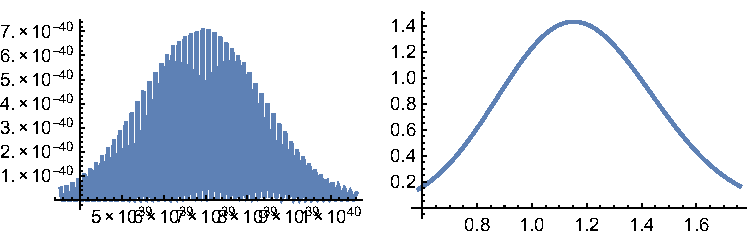
\includegraphics[width=0.48\textwidth]{hedgehog}
  \caption{Left: Prediction $p(\Lumtot \cond  \nu,  \npack, \bmnu, \bml)$, right: $p(x \cond  \nu,  \npack, \bmnu, \bmx)$. I sum over $N$ in both cases. }
  \fred{I still need to pretty this up. I used the old binned approach
    with 50 samples in a bin from which I computed the mean and
    variance to plug into \refeq{gmr} but I computed the sum over $N$
    instead of the integral.}
\label{fig:hedgehog}
\end{figure}

We chose the Gamma distribution because it is \emph{stable}; i.e.,
the sum of $N$ Gamma variates is again a Gamma variate
\begin{align}
  \lleq{gmb}
    X_j \sim \GammaDist(\alpha, \beta) \Rightarrow X \equiv \sum_{j=1}^N X_j \sim \GammaDist(N \alpha, \beta).
\end{align}
Assuming $\alpha = \alpha(\nu \cond \bmphi)$ and $\beta = \beta(\nu
\cond \bmphi)$ are functions of $\nu$ that depend on parameters
$\bmphi$, we set
\begin{align}
  \lleq{gmib}
  p(\bmX \cond \bmphi, N, \nu) &= \prod_{j=1}^N \GammaDist(X_j \cond \alpha, \beta ),\\
  p(\bmx \cond \bmphi, \npack, \bmnu) &= \prod_{i=1}^{\npack} \GammaDist(x_i \cond \alpha_i, \beta_i).
\end{align}
where $\alpha_i \equiv \alpha(\nu_i \cond \bmphi), \beta_i \equiv
\beta(\nu_i \cond \bmphi)$.

\subsection{Linear model}

\fred{Parts may still be relevant, especially if we put a plot of an
  entire spectrum in the paper.}

For simple functions $\alpha(\nu \cond \bmphi)$, one can find the
minimum value of $\alpha$ over the entire range of $\nu$
analytically. If this is too complicated, we propose to require
$\alpha(\nu_i \cond \bmphi) > 1$ only at each packet frequency
$\nu_i$. In the evaluation of $p(\bmx \cond \bmphi, \npack, \bmnu)$,
one has to loop over all packets and compute $\alpha$ and $\beta$
anyways, so the constraint imposes essentially no computational
overhead.


In the absence of a physical model to determine
$\alpha(\nu \cond \bmphi)$ and $\beta(\nu \cond \bmphi)$, we propose
to start with a simple polynomial ansatz
$\alpha(\nu \cond \bmphi) = \sum_{k=0}^\Kalpha \alpha_k \nu^k,
\beta(\nu \cond \bmphi) = \sum_{k=0}^\Kbeta \beta_k \nu^k$ such that
\begin{align}
  \lleq{gmp}
  \bmphi = (\alpha_0, \dots \alpha_\Kalpha , \beta_0, \dots \beta_\Kbeta)
\end{align}
The usual trade off between parsimony and the ability to accurately
model the frequency dependence determines the orders of the
polynomials, $\Kalpha$ and $\Kbeta$. This is outside the scope of this
paper. Here we choose $\Kalpha = 3$ and $\Kbeta = 1$.

%%%%%%%%%%%%%%%%%%%%%%%%%%%%%%%%%%%%%%%%%%%%%%%%%%%%%%%%%%%%%%%%%%%%%%%%%
\section{Asymptotic approximation} \label{sec:asymptotic}

\subsection{Derivation of $p(Q\,|\,n,\boldmath{\ell})$ for large $n$}

We return to the general formulation of \refeq{sll} and re-arrange its
factors into
\begin{align}
  \lleq{asc}
  p(Q\cond n,\bml)
  &= \int \rmdx{\lambda}\; \rmdx{\bmphi}\;
    p(\lambda\cond n)\;
    p(\bmphi\cond n,\bml)\;
    p(Q\cond \lambda,\bmphi) \\
  \lleq{asd}
  p(Q\cond \lambda,\bmphi)
  &= \sum_N
    p(N\cond \lambda)\;
    \int \rmdx{\bmL}\;
    p(Q\cond N,\bmL)\;
    p(\bmL\cond n,\bmphi)
\end{align}
with $p(\bmL\cond n,\bmphi) = \prod_{j=1}^n p(L_j\cond\bmphi)$ as
before. Again all quantities are related to a single bin in frequency.
Writing the moments and variance of $L$ as\footnote{The $k$-th moment
  of variable $x$ is defined as the expectation value $\mu_k =
  \expect{x^k} = \int \rmdx{x}\,x^k\,p(x),\; k = 0,1,2,\ldots$.} %
\begin{align}
  \lleq{ram}
  \mu =  \mu_1 &\equiv \expect{\Lum}, \qquad
  \mu_2 \equiv \expect{\Lum^2}, \\
  \sigma^2 &\equiv \variance{\Lum}
  = \expect{\Lum^2} - \expect{\Lum}^2,
\end{align}
it is easy to show that, for the Poissonian compound process
(\ref{asd}), the first moment and variance of $Q$ are related to those
of $L$ by
%%%%%%%%%%%%%%%%
\fredmargin{citation} %
%%%%%%%%%%%%%%%
\begin{align}
  \lleq{raa}
  \expect{Q} = \lambda \mu, \qquad
  \variance{Q} = \lambda \mu_2 = \lambda (\mu^2 + \sigma^2) \,.
\end{align}
for any probability $p(L\cond\bmphi)$.
%
Higher-order quantities such as the skewness and kurtosis
are suppressed by powers of $\lambda^{-1/2}$.
%%%%%%%%%%%
\hans{The variance is the second so-called \textit{cumulant}. The
  relation for all orders is that the $k$-th order cumulant
  $\kappa_q(Q)$ is equal to $\lambda$ times the $k$-th order moment of
  $L$, $\mu_k$. The skewness is therefore
  $\kappa_3(Q)/\kappa_2(Q)^{3/2} = \lambda \mu_3/(\lambda \mu_2)^{3/2}
  = \lambda^{-1/2} \mu_3/\mu_2^{3/2}$. The magnitude of the correction
  to (rab) due to $\kappa_3$ and higher orders is unclear.}
%%%%%%%%%%%
From Theorem 4.3.1 of Ref.~\cite{bening2002generalized}, we conclude
that the asymptotic distribution of $\Lumtot$ when
$\lambda \to \infty$, given the first and second moment of $\Lum$, is
a gaussian or normal distribution,
\begin{align}
  \lleq{rab}
  P(\Lumtot \cond \lambda,\bmphi)
  &= \GaussianDist \left( \Lumtot \cond \expect{Q}, \variance{Q} \right) %
    = \GaussianDist \left( \Lumtot \cond \lambda \mu_1, \lambda (\mu^2 {+} \sigma^2) \right).
\end{align}
This drastic simplification eliminates both the sum over $N$ and the
integral over $\bmL$ in \refeq{asd}.

It remains to find the integrals over $\lambda$ and $\bmphi$ in
\refeq{asc}. As before, the posterior for $\lambda$ is the Gamma
distribution of \refeq{pms}. %
%
To determine $p(\bmphi\cond n,\bml)$, we note that the result
(\ref{rab}) also simplifies the calculation of the parameter posterior
$p(\bmphi\cond n,\bml)$ since, independently of the actual functional
model for $p(L\cond\bmphi)$ the only relevant information is contained
in the first moment $\mu$ and variance $\sigma^2$.  As set out in
Jaynes~\cite[Ch. 7.10]{jaynes2003probability}, knowledge of $\mu$ and
$\sigma^2$ implies that we can assign a Gaussian distribution to
$p(L\cond\bmphi)$
\begin{align}
  \lleq{rae}
  p(\Lum \cond \bmphi) =
  p(\Lum \cond \mu, \sigma^2 ) &= \GaussianDist(\Lum \cond \mu, \sigma^2)
\end{align}
even though the actual data histograms may not be Gaussian. The reason
is that a Gaussian represents our state of knowledge \emph{before}
data $\bmy$ is observed. With this assignment, the definition of
$\bmphi$ reduces to $(\mu,\sigma^2)$ and the posterior becomes, using
Bayes' Theorem,
\begin{align}
  \lleq{rac}
  p(\mu,\sigma^2\cond n,\bml)
  &= \frac{
    \GaussianDist(\bml\cond\mu,\sigma^2)\;
    p(\mu\cond n)\;
    p(\sigma^2\cond n)}
  {p(\bml\cond n)}
\end{align}
\hans{I have inserted a uniform prior for $\mu$ here; see comments
  below. The original Gaussian prior has been retained below but I
  would suggest that the compliations introduced by it are
  unnecessary.}  %
In keeping with prior information that luminositites are always
positive, we assign an improper uniform prior
$p(\mu\cond\mu_{\rm max}) = 1/\mu_{\rm max}$ independent of $n$; as
always, the posterior is independent of $\mu_{\rm max}$. For
$\sigma^2$, we use an $n$-independent Inverse Gamma distribution prior
with hyperparameters $(a_0,b_0)$ which reads
\begin{align}
  \lleq{rad}
  p(\sigma^2\cond a_0,b_0)
  = \InvGammaDist(\sigma^2\cond a_0,b_0)
  &= \frac{b_0^{a_0}}{\Gamma(a_0)} (\sigma^2)^{-a_0-1} \exp(-b_0/\sigma^2)
\end{align}
and is ``conjugate'' to the normal distribution likelihood of
\refeq{rae} in that the posterior for $(\mu,\sigma^2)$ is also a
Gaussian in $\mu$ and an Inverse Gamma in $\sigma^2$, but with
parameters updated by the data,
\begin{align}
  \lleq{rbd}
  p(\mu,\sigma^2\cond n,\bml,a_0,b_0)
  &= \GaussianDist(\mu\cond \mu_n,\sigma_n^2)
  \cdot
  \InvGammaDist(\sigma^2\cond a_n,b_n) \\
  \mu_n &= \langle\ell\rangle\\
  \sigma_n^2 &= \sigma^2/n \\
  a_n &= a_0 + \tfrac{1}{2}n \\
  b_n &= b_0 + \tfrac{1}{2} n\left( \langle\ell^2\rangle - \langle\ell\rangle^2\right)
\end{align}
with data sample moments $\langle\lum^k\rangle$ defined as $(1/n)
\sum_{j=1}^n \lum_j^k$.
%
Inserting Eqs.~(\ref{pms}) and (\ref{rbd}) into \refeq{asc}, we obtain
\begin{align}
  \lleq{ral}
  p(\Lumtot \cond n,\bml)
  &= \int \rmdx{\lambda}\; \rmdx{\mu}\; \rmdx{\sigma^2}\;
  \GaussianDist \left( \Lumtot \cond \lambda \mu, \lambda (\sigma^2{+}\mu^2) \right)
  \times\\
  &\quad\times
  \GammaDist(\lambda \cond n{-}a{+}1 , 1) \cdot
  \GaussianDist(\mu\cond \mu_n,\sigma_n^2) \cdot
  \InvGammaDist(\sigma^2\cond a_n,b_n) \;
  \nonumber
\end{align}
While the integral cannot be carried out analytically, the integrand
is unimodal and strongly peaked, so that the Laplace or saddle-point
approximation~\cite[Ch. 27]{mackay2003information} can be applied.
%%%%%%%%%%%%%%%%%%%%%%%%%%%
\hans{Some comments on the numerical values of hyperparameters $a$ in Poisson, $a,b$
  in inverse gamma needed.} %
\hans{I would omit the text and calculations below. Apart from the
  extra parameters, the main reason is that the Gaussian prior in
  $\mu$ is not consistent with the fact that all luminosities are
  positive, while the gaussian permits negative $\mu$. This may not be
  important numerically, but the uniform prior in $\mu$ does
  circumvent this problem and is moreover less informative than the
  Gaussian prior. } %
\hans{Note also that letting $\mu_0{=}0$ and $ n_0\to 0$ below implies
  a prior gaussian of infinite width centered on zero, i.e.\ half of
  the values of $\mu$ will be negative. Could this be the reason why
  the numerics pick up a factor two?}
%%%%%%%%%%%%%%%%%%%%%%%%%%%


To simplify the calculations, we assume a conjugate prior for unknown
$\mu$ and $\sigma^2$. The standard result for the posterior is a
Gaussian for $\mu$ and an Inverse Gamma distribution for $\sigma^2$,
\begin{align}
  \lleq{raf}
  p(\mu, \sigma^2 \cond \bmy)
  &= \GaussianDist\left(\mu \cond \mu_0^\prime, \sigma^2/n_0^\prime\right) %
    \InvGammaDist\left( \sigma^2 \,\Bigl|\, \tfrac{1}{2}\nu_0^\prime,
    \tfrac{1}{2}\nu_0^\prime \sigma_0^{\prime 2} \right)
\end{align}
where the hyperparameters $(n_0',\mu_0',\nu_0')$ are updated from
prior to posterior based on $\bmy$ with the sample mean
$\langle\lum\rangle = (1/n) \sum_{j=1}^n \lum_j$,
\begin{align}
  %\lleq{rag}
  \lleq{rah}  n_0^\prime
  &= n_0 + n,\\
  \lleq{rai}    \mu_0^\prime
  &= \frac{n_0 \mu_0 + n \langle\lum\rangle}{n_0^\prime},\\
  \lleq{raj}    \nu_0^\prime
  &= \nu_0 + n,\\
  \lleq{rak}
  \nu_0^\prime \sigma_0^{\prime 2}
  &= \nu_0 \sigma_0^{ 2}
    + \sum_{j=1}^n \left(\lum_j - \langle\lum\rangle\right)^2
    + \frac{n_0 n}{n_0^\prime} \left(\mu_0 - \langle\lum\rangle\right)^2\,.
\end{align}
By default, we take a noninformative prior and set $n_0 = \mu_0 =
\nu_0 = 0$, so the value $\sigma_0^2>0$ is irrelevant. %
  % The posterior
  % $ p(\expect{\Lum}, \expect{\Lum^2} \cond \bmy)$ is given by
  % \refeq{raf} with $\mu, \sigma^2$ replaced by
  % $\expect{\Lum}, \expect{\Lum^2}$ as indicated in \refeq{rae} because
  % the Jacobian determinant is one.
The above equations also show that the data $\bmy$ appear only in the
form of $n$ and the first two sample moments
$m_1 = \langle\ell\rangle$ and $m_2 = \langle\ell^2\rangle$.
Inserting all these ingredients into Eq.~(\ref{asc}), we obtain
\begin{align}
  \lleq{ral}
  p(\Lumtot \cond \bmy)
  &= \int \rmdx{\lambda}\; \rmdx{\mu}\; \rmdx{\sigma^2}\;
    p(\lambda \cond n)\; p( \mu, \sigma^2 \cond \bmy)\;
    \GaussianDist \left( \Lumtot \cond \lambda \mu, \lambda (\sigma^2{+}\mu^2) \right)
    \,,
\end{align}
where $ p(\lambda \cond n)$ is given by \refeq{pms} and
$ p( \mu, \sigma^2 \cond \bmy)$ by Eqs.~(\ref{raf})--(\ref{rak}).

\subsection{Numerical implementation}\label{sec:asympt-numeric}

\hans{H: If threefold integrals must be carried out for the
  expectation values, why not do so for Eq (ral) directly rather than
  just the expectation values?} %

While the integral in \refeq{ral} cannot be integrated analytically,
the integrand is unimodal and strongly peaked, so that the Laplace or
saddle-point approximation~\cite[Ch. 27]{mackay2003information} can be
applied. If only the value $p(\Lumtot{=}\lumtot \cond n,m_1,m_2)$ at the
total data luminosity $q$ is sought, then one can approximate it
directly. In addition, we can compute the moments of $\Lumtot$ through
the \emph{moment generating function} \cite{stuart1994kendall}
\begin{align}
  \lleq{rap}
  M(t \cond \bmy) = \int_0^{\infty} \rmdx{\Lumtot} p(\Lumtot \cond \bmy) e^{-t \Lumtot} \,
\end{align}
from which the moments are accessible by differentiation
\begin{align}
  \lleq{raq}
  \expect{\Lumtot^k} = (-1)^k \eval{\dv[k]{M(t \cond \bmy)}{t}}_{t=0}
\end{align}
Assuming all involved integrals are absolutely convergent, we can
exchange the order of integration and find
\begin{align}
  \lleq{rar}
  M(t \cond \bmy) &= \int \rmdx{\lambda} \rmdx{\mu} \rmdx{\sigma^2} p(\lambda \cond \bmy) p( \mu, \sigma^2 \cond \bmy)  f(t \cond \lambda, \mu, \sigma^2),
  \intertext{where }
  f\left(t \cond  \lambda, \mu, \sigma^2\right) &\equiv \int \rmdx{\Lumtot} \GaussianDist \left( \Lumtot \cond \lambda \mu, \lambda \sigma^2 \right) e^{-t \Lumtot}= \frac{1}{2} e^{t \lambda (t \sigma^2/2 - \mu)} \left[ 1 + \erf\qty( \frac{\sqrt{\lambda}(\mu - t \sigma^2)}{\sqrt{2 \sigma^2}}) \right].
\end{align}
This implies that the mean and variance of $\Lumtot$ require an integral over the three parameters
\begin{align}
  \lleq{ras}
  \expect{\Lumtot} &= \int \rmdx{\lambda} \rmdx{\mu} \rmdx{\sigma^2} p(\lambda \cond n) p( \mu, \sigma^2 \cond \bmy) \qty(-\eval{\dv{f(t \cond  \lambda, \mu, \sigma^2)}{t}}_{t=0})\\
  \variance{\Lumtot} &= \int \rmdx{\lambda} \rmdx{\mu} \rmdx{\sigma^2} p(\lambda \cond n) p( \mu, \sigma^2 \cond \bmy) \qty(\eval{\dv[2]{f(t \cond  \lambda, \mu, \sigma^2)}{t}}_{t=0}) - \expect{\Lumtot}^2
\end{align}
We implemented the above formulae in the julia language~\cite{julia14}
and used Newton's method from the \texttt{Optim.jl} package in
combination with automatic
differentiation~\cite{RevelsLubinPapamarkou2016} to optimize the
respective integrand and compute the Hessian at the mode. As initial
values, we slightly offset the sample estimates to avoid issues if the
optimizer cannot improve on the initial guess and found convergence
within $\order{10}$ steps:
\begin{align}
  \lleq{rat}
  \qty(\lambda, \mu, \sigma^2) = 1.0005 (n, \langle\lum\rangle, \langle\lum^2\rangle{-}\langle\lum\rangle^2).
\end{align}
\fred{Did we define expectation value and variance? Should be in notation or intro section. Hans: see footnote 2.} %
\fred{At least for us, I should do a comparison plot to evaluate $p(\Lumtot \cond \bmy)$ with both methods } %
\fred{We need a plot, the one to compare predictions and 250 real replicas or 100 virtual replicas?} %
\fred{Advantage of this approach: no need to store all packets anymore, sum and sum of squares can be accumulated online $\Rightarrow$ reduced computation and storage requirements}

\section{Conclusion} \label{sec:conclusion}

TODO

\section{Appendix} \label{sec:appendix}

\fred{Will be removed later}

We use the shorthand $\alpha_n \equiv \alpha(\nu_n \cond
\bmphi), \beta_n \equiv \beta(\nu_n \cond \bmphi), \alpha \equiv
\alpha(\nu \cond \bmphi), \beta \equiv \beta(\nu \cond \bmphi)$.

\subsection{Gradients} \label{sec:gradients}

\begin{align}
  \label{eq:grad-posterior}
  \left( \firstDeriv{\alpha_i}, \firstDeriv{\beta_i} \right) \log p(\bmx \cond \alpha, \beta) &=
  \left(
    \sum_n \left[ \log \beta_n - \Psi(\alpha_n) + \log x_n \right] \nu_n^i \;,
    \sum_n \left[ \frac{\alpha_n}{\beta_n} - x_n \right]\nu_n^i
  \right)
\end{align}

\begin{align}
  \label{eq:grad-prediction}
  \left( \firstDeriv{\alpha_i}, \firstDeriv{\beta_i}, \firstDeriv{N} \right) \log p(X \cond N \alpha, \beta)  &=
  \left(
    \left[ \log \beta - \Psi(N \alpha) + \log X \right] N \nu^i,
    \left[ \frac{N\alpha}{\beta} - X \right]\nu^i,
    \left[ \log \beta -\Psi(N \alpha) + \log X \right] \alpha
  \right)
\end{align}

\begin{align}
  \label{eq:grad-nb}
  \firstDeriv{N} \log p(N \cond n) = \Psi(N+n-a+1) - \Psi(N+1) - \log 2
\end{align}

\subsection{Hessians} \label{sec:hessians}

\begin{align}
  \label{eq:hess-posterior}
    - \left(
    \begin{array}{ccc}
      \secPartial{\alpha_i}{\alpha_j} & \secPartial{\alpha_i}{\beta_j}\\
      \dots & \secPartial{\beta_i}{\beta_j}
    \end{array}
  \right) \log p(\bmx \cond \alpha, \beta)
    &= \left(
    \begin{array}{cc}
      \sum_n \Psi'(\alpha_n) \nu_n^{i+j} & -\sum_n \frac{\nu_n^{i+j}}{\beta_n}\\
      \dots & \sum_n \frac{\alpha_n}{\beta_n^2} \nu_n^{i+j}
    \end{array}
  \right)
\end{align}

 \begin{align}
  \label{eq:hess-prediction}
  & - \left(
    \begin{array}{ccc}
      \secPartial{\alpha_i}{\alpha_j} & \secPartial{\alpha_i}{\beta_j} & \secPartial{\alpha_i}{N}\\
      \dots & \secPartial{\beta_i}{\beta_j} & \secPartial{\beta_i}{N}\\
      \dots & \dots & \secDeriv{N}
    \end{array}
  \right) \log p(X \cond N \alpha, \beta)
  \\
  &=
  \left(
    \begin{array}{ccc}
      N^2 \Psi'(N \alpha) \nu^{i+j} & -\frac{N \nu^{i+j}}{\beta} & \left[ -\log \beta +\Psi(N \alpha) + N \alpha \Psi'(N \alpha) - \log X \right] \nu^{i}\\
      \dots &  \frac{N\alpha}{\beta^2} \nu^{i+j} & -\frac{\alpha}{\beta} \nu^{i} \\
      \dots & \dots & \alpha^2 \Psi'(N \alpha)
    \end{array}
  \right)
\end{align}
\begin{align}
  \label{eq:hess-nb}
   - \secDeriv{N} \log p(N \cond n) = \Psi'(N+1) - \Psi'(N+n-a+1)
\end{align}

\bibliographystyle{plain}
\bibliography{references}

\end{document}

% Local Variables:
% compile-command:"rubber --pdf -W refs --synctex draft"
% End: